\documentclass{beamer}
% Introdução ao LaTeX
% LaTeX Básico
% Geraldo Xexéo
% Este arquivo tem a licença Creative Commons
% BY-NC-SA 2020
%\usepackage[utf8]{inputenc}
\usepackage[T1]{fontenc}
\usepackage[english,brazilian]{babel}
\usepackage{graphicx}
\usepackage{hologo}
\usepackage{outlines}
\usepackage{listings}
\usepackage[style=brazilian]{csquotes}
\usepackage{xpatch}
% to use \currenttime
\usepackage{datetime}





\usetheme{Luebeck}
\mode<presentation>
\setbeamertemplate{page number in head/foot}[totalpagenumber]
%\logo{\includegraphics[height=0.8cm]{Images/Logo_LUDES_FINAL_CORES-02.png}\vspace{220pt}}
\AtBeginSection[]
{
  \begin{frame}
    \frametitle{Onde Estamos?}
    \tableofcontents[currentsection,hideallsubsections ]
  \end{frame}
}

%\addtobeamertemplate{frametitle}{}{%
%    \begin{textblock*}{0mm}(-.09\textwidth,-2cm)
%        
\includegraphics[height=0.7cm]{Images/LINE.png}
%    \end{textblock*}
%    \begin{textblock*}{0mm}(.85\textwidth,-2cm)
%        
\includegraphics[height=0.7cm]{Images/LUDES1.png}
%\end{textblock*}}


\title{\LaTeX\ Básico}
\subtitle{Seminário \LaTeX\ - Parte III}


\author{Geraldo Xexéo\inst{1,2}}

\institute[DCC/PESC]{\inst{1}Departamento de Ciências da Computação 
\and
\inst{2}Programa de Engenharia de Sistemas e Computação}

\date[LUDES/LINE]{3o Seminário LUDES/LINE, Março 2020}



\begin{document}


\begin{frame}
\titlepage
\centering
%
\includegraphics[width=.6\linewidth]{Images/Logomarcas.png}
\end{frame}

\begin{frame}
\frametitle{Agenda}
\tableofcontents[hideallsubsections]
\end{frame}

\begin{frame}{Bibliografia}
    Lamport, Leslie. \LaTeX, a Document Preparation System
    
    \begin{figure}
        \centering
        
\includegraphics[width=.3\linewidth]{Images/Picture6.jpg}
    \end{figure}
\end{frame}

\section{Motivação}



\subsection{WYSIAYG}
\begin{frame}
\frametitle{What you see is all you've got}
\begin{itemize}
    \item WYSIWYG: What you see is what you get
    \item What you see is all you´ve got
    \item O WYSIWYG faz o autor se preocupar com o design visual
    \item Ok para pequenos textos
    \item E se você quiser mudar um comportamento em todo um texto bem grande, como um livro?
    \end{itemize}
\end{frame}

\subsection{Design Lógico de Documentos}
\begin{frame}{Design Lógico de Documentos}
\begin{outline}
    \1 Não se preocupar com o formato enquanto escreve o documento
    
        \2 Isso é possível em vários processadores de texto por meio do uso de estilos, porém os usuários raramente usam os estilos ou os usam corretamente
        
        \2 Muitos usuários se perdem pensando no formato, quando isso pode ser feito só no final
    
            \3 Também é possível com os processadores com estilo
           
    \1 Pensar o documento como uma estrutura lógica, e que você trata com comandos
\end{outline}
\end{frame}

\section{\LaTeX\ Muito Básico}
\subsection{Documento Mínimo}
\begin{frame}[fragile]{Documento mínimo}
    \begin{block}{\LaTeX}
        \begin{verbatim}
            \documentclass[a4paper]{article}
            %isto é um comentário
            %preâmbulo
            %onde colocamos comandos
            \begin{document}
            %área de texto 
            Hello World!
            \end{document} 
        \end{verbatim}
    \end{block}
\end{frame}


\begin{frame}{Primeiro Resultado} 
    \begin{figure}
        \centering
        
\includegraphics[width=.6\linewidth]{minimo.pdf}
    \end{figure}
\end{frame}

\subsection{documentclass}
\begin{frame}{documentclass}
    \begin{outline}
        \1 Cada documento possui uma classe
        \1 Essa classe controla as principais características e a diagramação geral
        \1 Existem opções para as classes
        \1  Vamos usar a classe article
        \1  Existe uma classe para os documentos acadêmicos da Coppe
        \2  Cobre dissertação, tese, exame de qualificação e outras coisas
        \2 https://github.com/COPPE-UFRJ/CoppeTeX
        \2 https://github.com/COPPE-UFRJ/CoppeTeX/tree/master/dist
        \1  Existem centenas de classes, muitas com apenas pequenas modificações de outras
    \end{outline}
\end{frame}

\subsection{Classes Mais Usadas}
\begin{frame}{Classes Mais Usadas}
    \begin{outline}
        \1 article
        \2 Organiza o documento em sections
        \1 report
        \1 book
        \2 Organiza o documento em chapters      
     \end{outline}
\end{frame} 

\subsection{Estrutura de um Documento}
\begin{frame}{Estrutura de um Documento}
    \begin{itemize}
        \item \textbackslash part\{\} -- só para report e book
        \item \textbackslash chapter\{\} -- só para report e book
        \item \textbackslash section\{\}
        \item \textbackslash subsection\{\}
        \item \textbackslash subsubsection\{\}
        \item \textbackslash paragraph\{\}
        \item \textbackslash subparagraph\{\}
    \end{itemize}
\end{frame}

\subsection{Informação de Capa}
\begin{frame}{Informação de Capa}
    \begin{itemize}
        \item \textbackslash title\{\}
        \item \textbackslash author\{\}
        \item \textbackslash date\{\}
    \end{itemize}
\end{frame}


\subsection{Meu Primeiro Artigo}
\begin{frame}[fragile]{Meu Primeiro Artigo}
    \begin{verbatim}
\documentclass{article}
\title{Um Artigo Mínimo}
\author{Geraldo Xexéo}
\begin{document}
\maketitle
\section{A primeira seção}
Lorem ...  augue. 
\section{A segunda seção}
Lorem ... augue.
\subsection{Um subseção}
Sed ... erat.
\end{document}    
\end{verbatim}
\end{frame}

\begin{frame}{Primeiro Artigo} 
    \begin{figure}
        \centering
        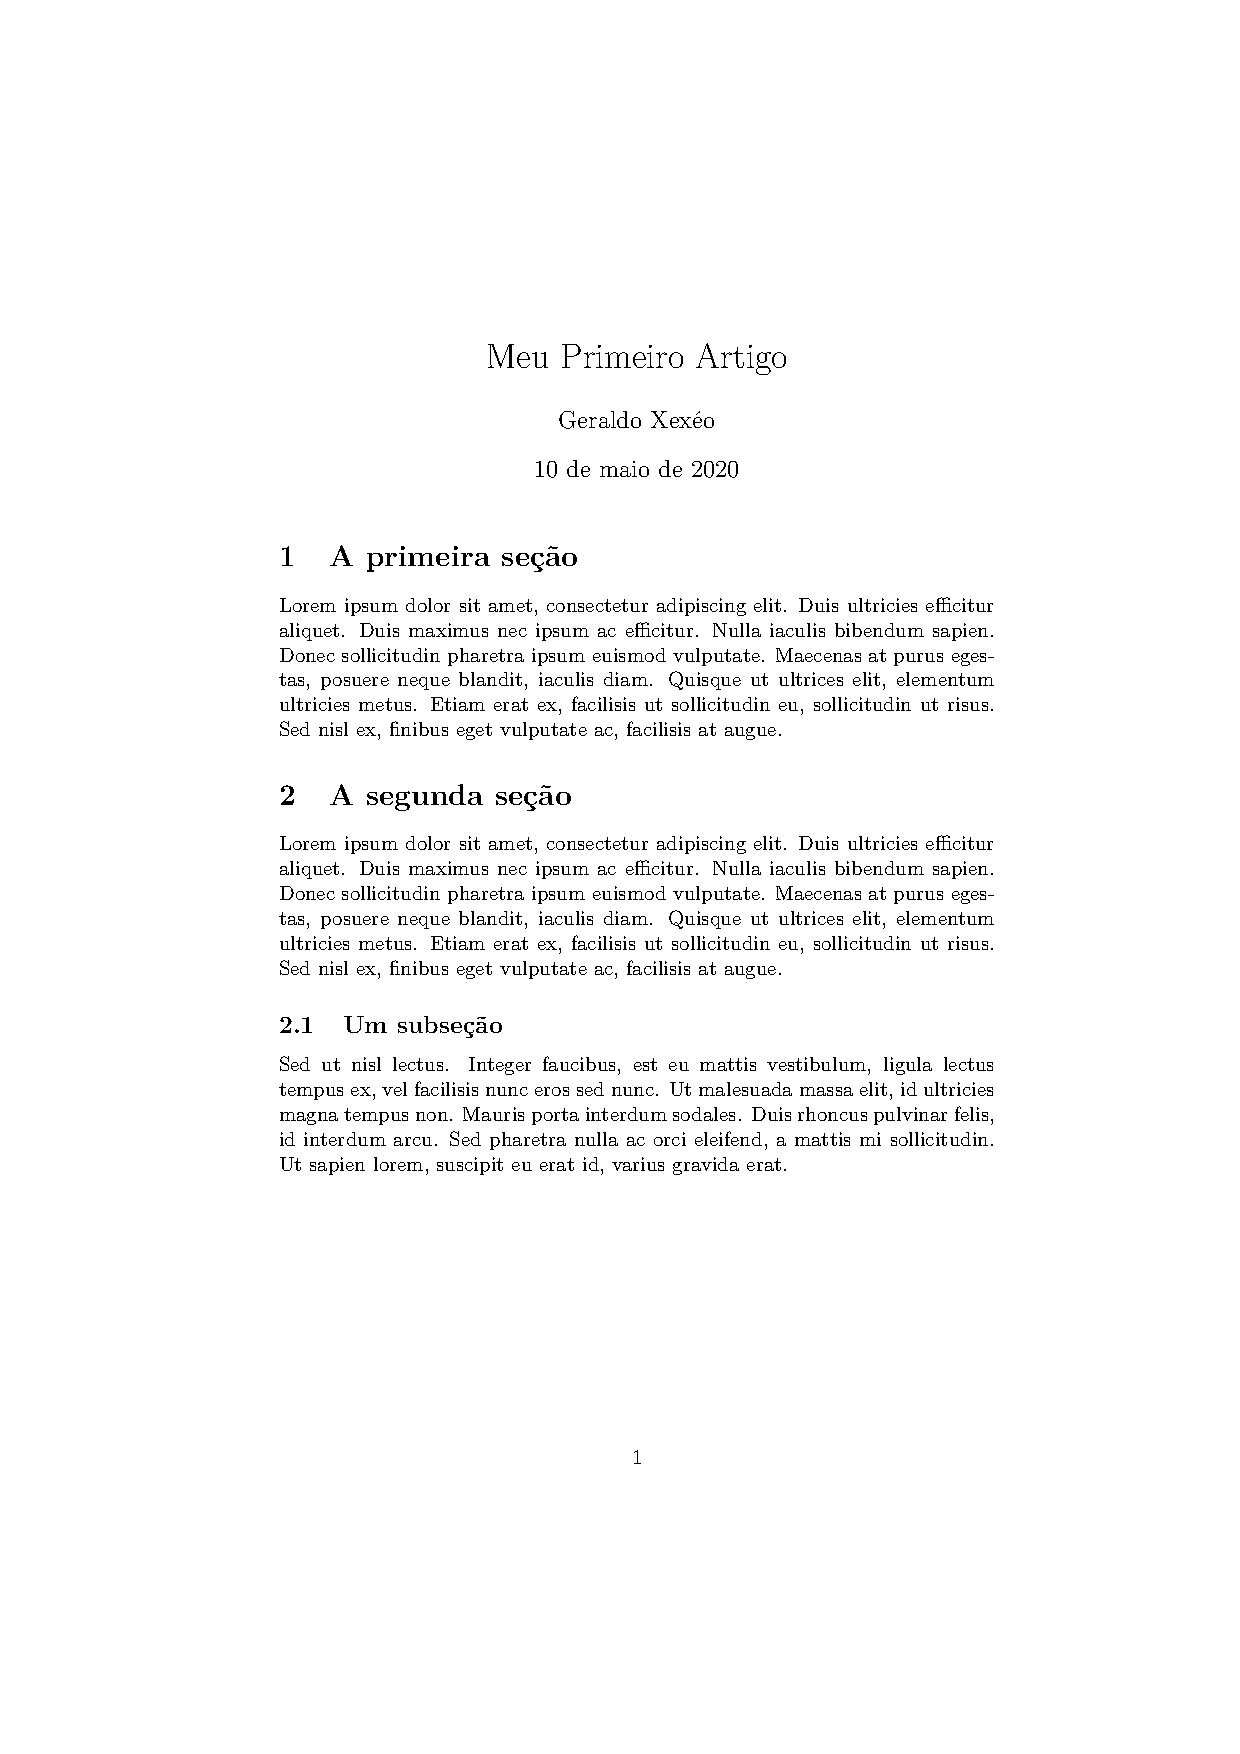
\includegraphics[width=.6\linewidth]{primeiroartigo.pdf}
    \end{figure}
\end{frame}


\subsection{Coloca o Resumo!}
\begin{frame}[shrink=10,fragile]{Coloca o Resumo!}
    \begin{verbatim}
    \documentclass{article}
    \title{Um Artigo Mínimo}
    \author{Geraldo Xexéo}
    \begin{document}
    \begin{abstract}
    Esse é o resumo, mas tá abstract!
    \end{abstract}
    \maketitle
    \section{A primeira seção}
    Lorem ...  augue. 
    \section{A segunda seção}
    Lorem ... augue.
    \subsection{Um subseção}
    Sed ... erat.
    \end{document}    
    \end{verbatim}
\end{frame}

\begin{frame}[t]{Algo Errado?} 
    \begin{figure}
        \centering
        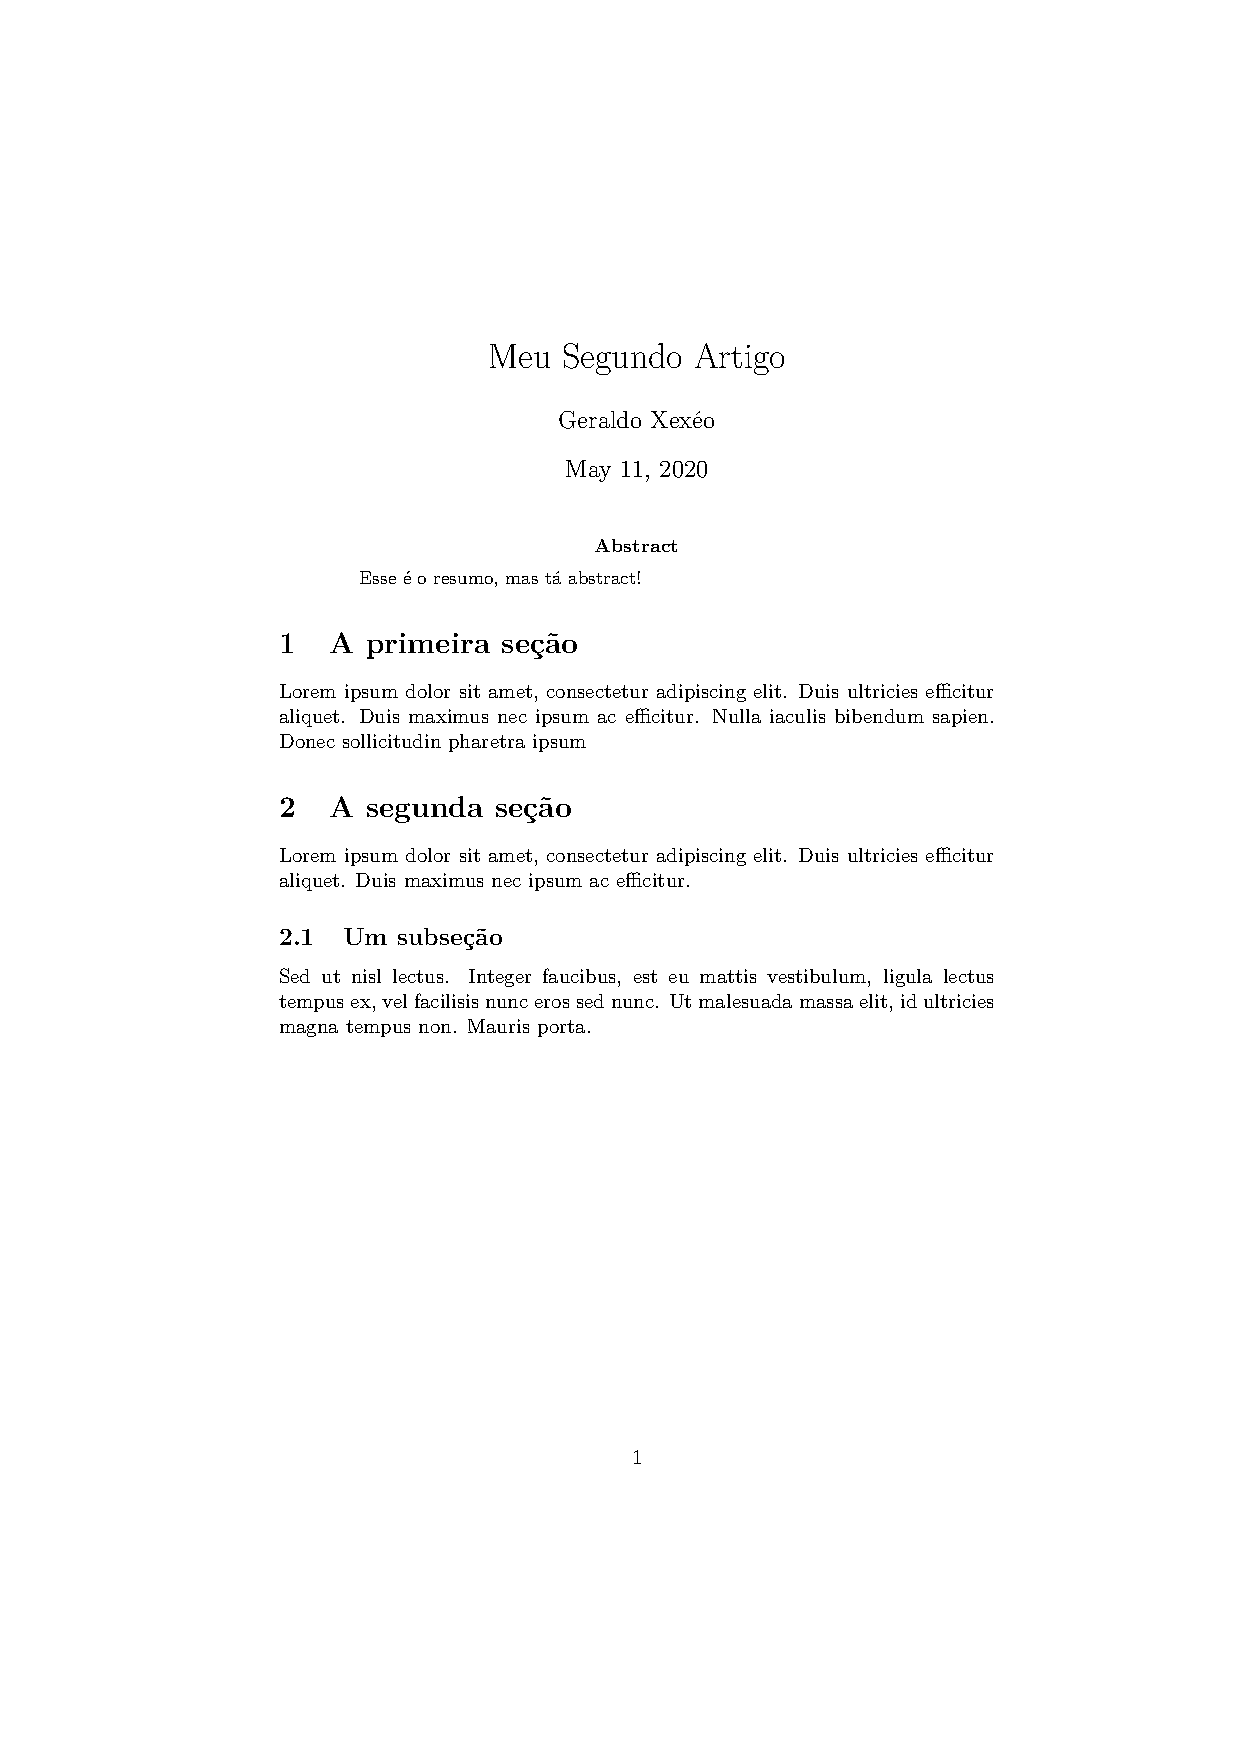
\includegraphics[width=.6\linewidth]{arquivocomabstract.pdf}
    \end{figure}
\end{frame}



\section{Comandos Mais Comuns}


\subsection{Formatar o Texto}
\begin{frame}{Formatar o Texto}
    \begin{columns}
        \begin{column}{0.5\linewidth}
                \begin{itemize}
                \item \textbackslash textbf\{negrito\}
                \item \textbackslash textit\{itálico\}
                \item \textbackslash underline\{sublinhado\}
                \item \textbackslash Large\{Grande\}
                \item e\textbackslash \^\ \{superscript\}
                \item e\textbackslash \_ \{subscript\}
            \end{itemize}
        \end{column}
                \begin{column}{0.5\linewidth}
            \begin{itemize}
                \item \textbf{negrito}
                \item \textit{itálico}
                \item \underline{sublinhado}
                \item \Large{Grande}
                \item e\textsuperscript{superscript}
                \item e\textsubscript{subscript}
            \end{itemize}
        \end{column}
    \end{columns}

\end{frame}

\subsection{Fazendo Referência a Outra Parte}
\begin{frame}{Fazendo Referência a Outra Parte}
    \begin{itemize}
        \item \textbackslash label\{\}
        \item \textbackslash ref\{\}
    \end{itemize}
\end{frame}

\begin{frame}[fragile]{Exemplo de Uso de Referência}
    \begin{verbatim}
\begin{document}

\maketitle

\section{A primeira seção}\label{sec:pri}

Leia a seção \ref{sec:seg}

\section{A segunda seção}\label{sec:seg}

Leia a seção \ref{sec:pri}
\end{document}
    \end{verbatim}
\end{frame}

\begin{frame}{Mostrando as Referências} 
    \begin{figure}
        \centering
        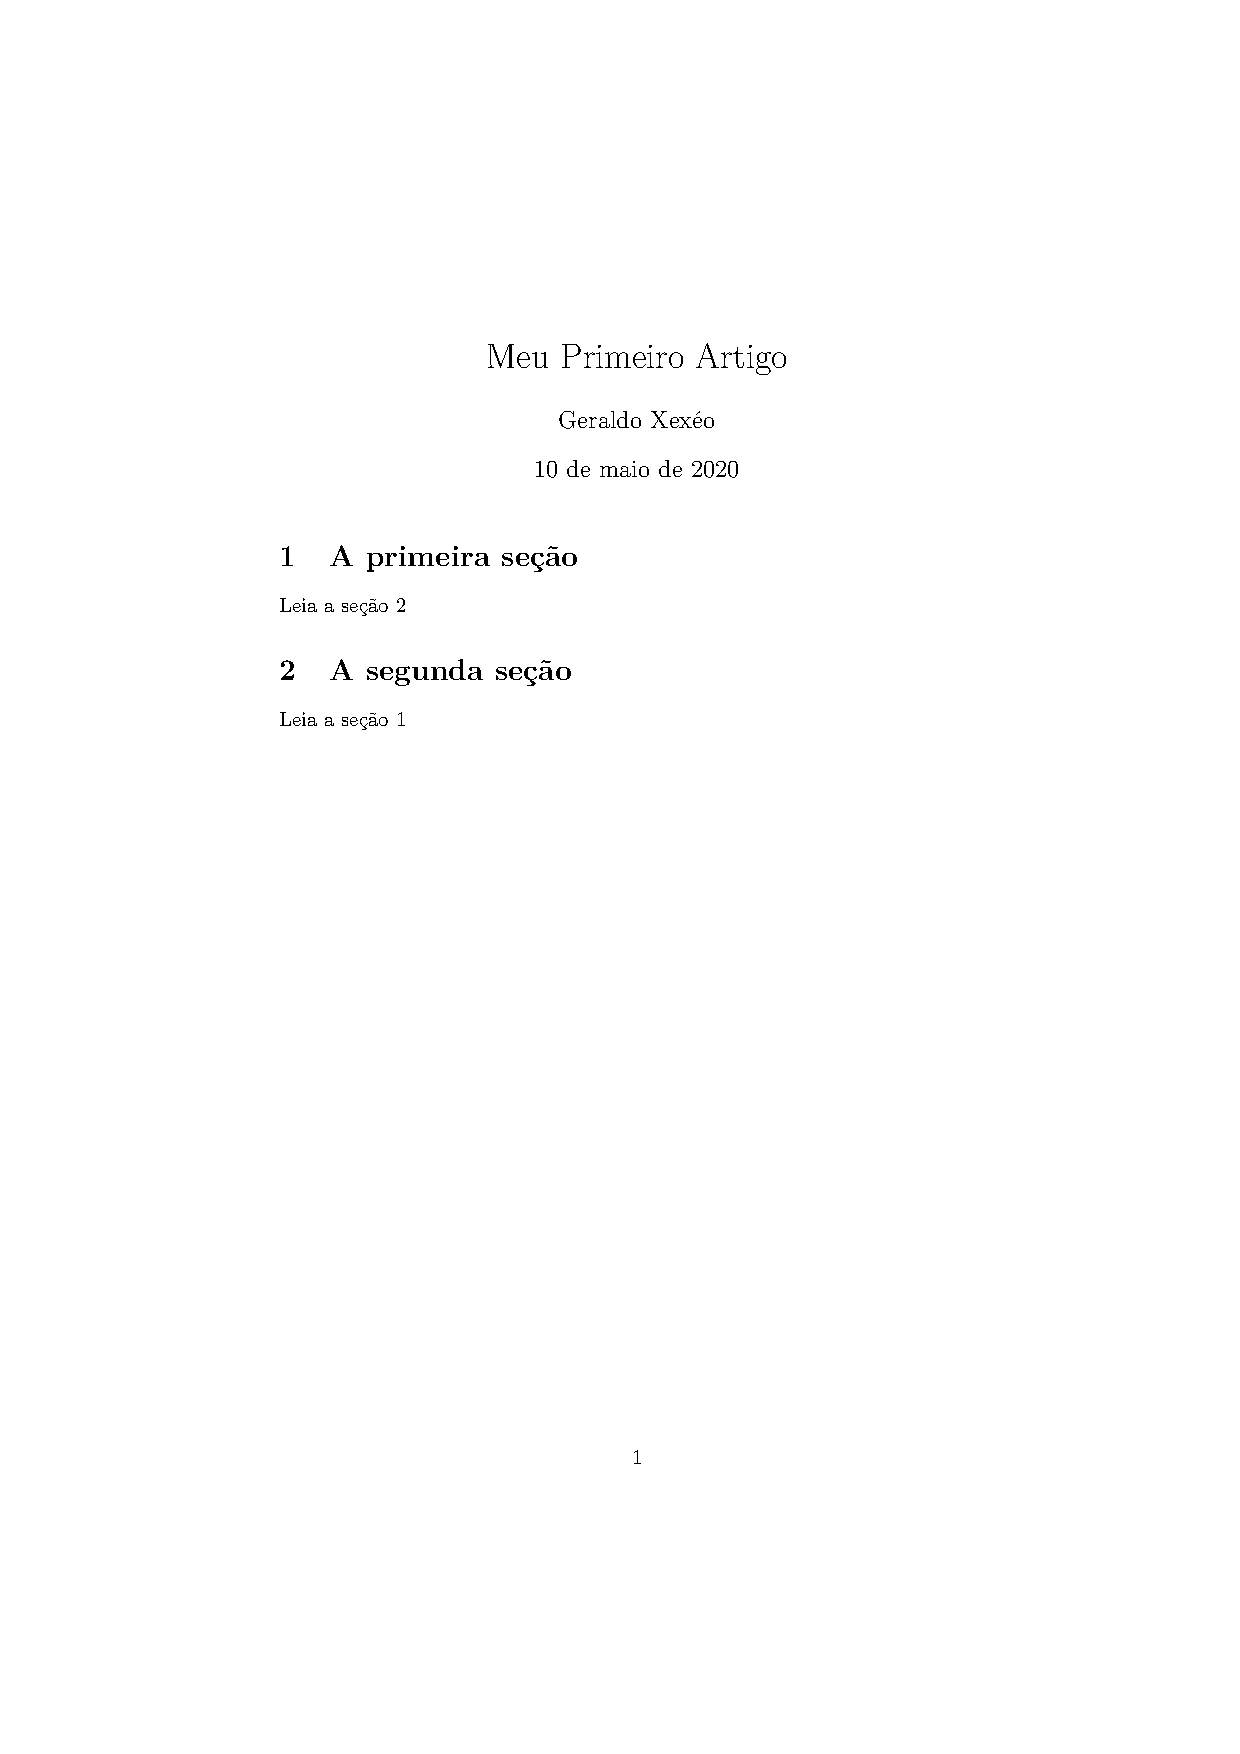
\includegraphics[width=.6\linewidth]{labelref.pdf}
    \end{figure}
\end{frame}






\section{Usando Pacotes}

\subsection{O Que São Pacotes}
\begin{frame}{O Que São Pacotes}
    \begin{outline}
        \1 São extensões que adicionam poder ao \LaTeX
        \1 Algumas são muito usadas
        \2 Babel -- para escrever em outras línguas
        \3 Sim, \LaTeX\ é muito focado em inglês, mas há muitos pacotes criados em outras línguas, como alemão.
        \3 Um bom pacote é auto-configurável na maioria das línguas por meio do Babel
        \3 Um ótimo pacote deixa você configurar como você quiser a língua
        \1 Comando 
        \2 \textbackslash usepackage{[opções]}\{pacote\}
        \1 Os bons pacotes tem várias formas de configurações nessas opções
        \1 Os bons pacotes estão vivos
    \end{outline}
\end{frame}


\subsection{Babel}
\begin{frame}{Babel}
    \begin{outline}
        \1 Pacote que permite usar o \LaTeX\ com outras linguagens
        \1 Chamado por pacotes que escrevem algo, como a palavra ``Capítulo''
        \1 Comando 
        \2 \textbackslash usepackage{[english,\textbf{brazilian}]}\{babel\}
        \2 A última linguagem é a mais importante
        \1 A opção ``portuguese'' usa termos de Portugal, como dizer que um documento Web foi \textit{acedido} em vez de \textit{acessado}.
        \1 Usar \textbf{brazilian}
    \end{outline}
\end{frame}

\subsection{inputencode}
\begin{frame}{inputencode}
    \begin{outline}
        \1 \textbackslash usepackage{[utf8]}\{inputencode\}
        \1 Faz o \LaTeX\ entender código UTF-8 nos documentos que ele lê
            \2 Caracteres acentuados do Português e outras línguas!
            \3 áéíóúâêîôûäëïöüàèìòù
        \1 Você não precisa mais usar \textbackslash´e
        \1 \textbf{Não use o utf8x}, ele morreu e tem defeitos
        \1 Melhor ainda, use o \hologo{LuaLaTeX} e dispense esse pacote!
    \end{outline}
\end{frame}

\subsection{fontencode}
\begin{frame}{fontencode}
    \begin{outline}
        \1 \textbackslash usepackage{[T1]}\{fontenc\}
        \1 Quando gera o PDF, o \LaTeX\ por \textit{default} use o \textit{font encoding} OT1, que só tem 7 bits.
        \2 Isso faz que uma leitura do texto do PDF para indexação, por exemplo, recupere combinações de caracteres que foram geradas para representar um caracter
        \3 Isso gera problemas na indexação do seu documento, ruim para você
        \1 Garante também que as ligaduras, grande parte da beleza do texto do \TeX\ sejam geradas, pois elas não são construídas, mas sim pertencentes as fontes.
        \1 Sempre necessário
    \end{outline}
\end{frame}

\section{Ambientes}
\subsection{O Que São Ambientes}
\begin{frame}{O Que São Ambientes}
\begin{itemize}
    \item Ambientes são escopos fechados que são usados para mudar, temporariamente, o comportamento do \LaTeX\
    \item Basicamente, um contexto
    \item tem início (\textbackslash begin\{nome\}) e fim (\textbackslash end\{nome\})
    \item Em geral, um comando dado dentro do ambiente deixa de ser válido fora do ambiente
    \item Tem que ser construídos um dentro do outro. São estruturados
\end{itemize}
\end{frame}

\subsection{Ambiente Mais Usados}
\begin{frame}[fragile]{Ambiente Mais Usados}
    \begin{columns}
        \begin{column}{0.3\linewidth}  
            \begin{outline}
                \1<1-> itemize
                \1<2-> enumerate
                \1<3-> equation
                \1<3-> Floats
                \2<3-> table
                \2<3-> figure
                \1<3-> tabular
                                
            \end{outline}
        \end{column}
        \begin{column}{0.3\linewidth}  
            \only<1>{\sffamily
                
            \textbackslash begin\{itemize\}
            
            ~~~\textbackslash item um 
               
            ~~~\textbackslash item dois
            
            ~~~\textbackslash item três
               
            \textbackslash end\{itemize\}
            }
            \only<2>{\sffamily
                
            \textbackslash begin\{enumerate\}
            
            ~~~\textbackslash item um 
                
            ~~~\textbackslash item dois
            
            ~~~\textbackslash item três
                
            \textbackslash end\{enumerate\}
        }
        \end{column}
            \begin{column}{0.3\linewidth}  
        \only<1>{
            Uma lista de itens:
            \begin{itemize}
              \item um 
                \item dois
                \item três
            \end{itemize}
        }
        \only<2>{\sffamily
            Uma enumeração:
            \begin{enumerate}
                \item um 
                \item dois
                \item três
\end{enumerate}
        }
    \uncover<3->{Vamos ver...}
    \end{column}
    \end{columns}


\end{frame}




\subsection{Equações}
\begin{frame}[fragile]{Equações...}
    Você pode fazer equações dentro do texto, usando \verb|$\frac{x!}{(x-n)!n!}$| que resulta em
$\frac{x!}{(x-n)!n!}$

Ou você pode usar um ambiente equation, como em 

\begin{verbatim}

\begin{equation}
\frac{x!}{(x-n)!n!}
\end{equation}

\end{verbatim}

que resulta em 

\begin{equation}
\frac{x!}{(x-n)!n!}
\end{equation}
\end{frame}



\subsection{Equações}
\begin{frame}[shrink=20,fragile]{Equações...} 
    \begin{verbatim}
\documentclass{article}
\usepackage[T1]{fontenc}
\title{Meu Terceiro Artigo}
\author{Geraldo Xexéo}
\begin{document}
\maketitle
Você pode fazer uma equação in line $\sin(\theta)^\pi)$ ou citar
a equação \ref{eq:cita} que vai ficar destacada no texto.
\begin{equation}\label{eq:cita}
y = \sum^{N}_{i=1} \cos(\alpha_i^\rho)+3\times \log(x)
\end{equation}
\end{document}
    \end{verbatim}
\end{frame}


\begin{frame}{Equações no artigo} 
    \begin{figure}
        \centering
        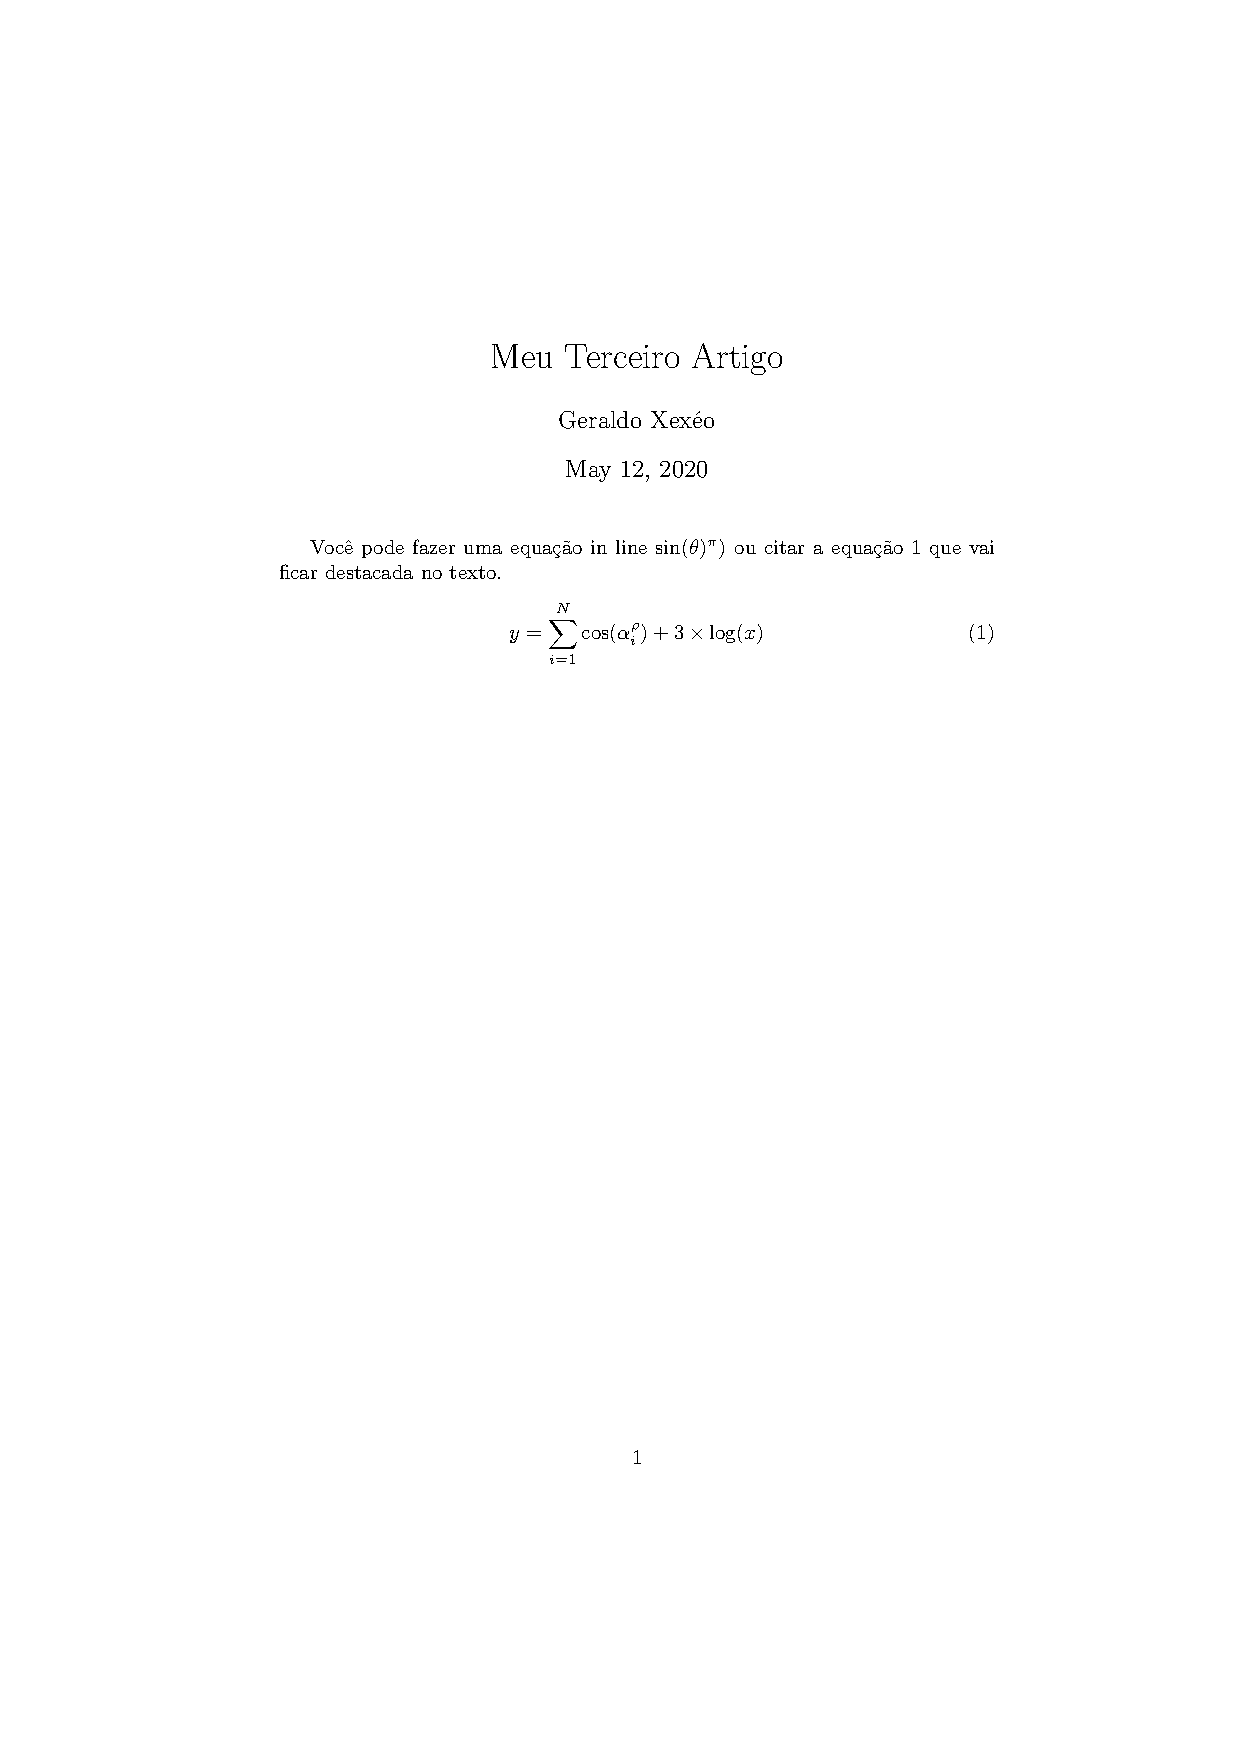
\includegraphics[width=.8\linewidth]{terceiroartigo.pdf}
    \end{figure}
\end{frame}

\subsection{Equações}
\begin{frame}{Aprendendo devagar as fórmulas}
Você pode aprender as fórmulas bem devagar, usando para isso
programas que escrevem elas para você.

https://latex.codecogs.com/eqneditor/editor.php

    \begin{figure}
    \centering
    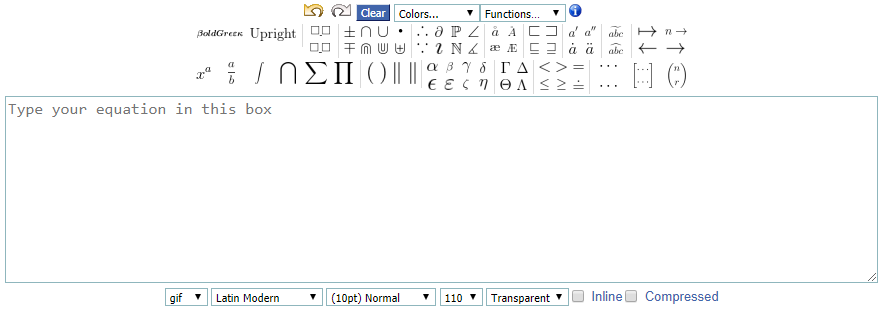
\includegraphics[width=.8\linewidth]{Images/equationeditor.png}
\end{figure}

\end{frame}

\section{Floats}
\subsection{O Que São Floats}
\begin{frame}{O Que São Floats}
    \begin{outline}
        \1 Ambientes que o \LaTeX\ posiciona no melhor lugar possível de acordo com suas regras de diagramação.
        \2 figure
        \2 table
        \1 Permite opções que orientam o algoritmo
        \2 \textbackslash \{figure\}[hbt]
        \3 here, bottom e top
        \2 Essa é a melhor ordem, pois (quase) garante que a imagem não vai aparecer antes de ser citada
        \1 Flutuam
        \2 Você não determina exatamente onde vão ficar
    \end{outline}
\end{frame}


\subsection{Figure}
\begin{frame}[fragile]{O ambiente figure}
\begin{verbatim}
\begin{figure}
    \centering
    
\includegraphics[height=0.5\textheight]{Images/Picture6}
    \caption{Capa do livro de \LaTeX\ }
    \label{fig:picture6}
\end{figure}
\end{verbatim}    
\end{frame}



\begin{frame}[fragile]{O ambiente figure}
\begin{figure}
    \centering
    
\includegraphics[height=0.5\textheight]{Images/Picture6}
    \caption{Capa do livro de \LaTeX\ }
    \label{fig:picture6}
\end{figure}
\end{frame}

\subsection{Table}
\begin{frame}[fragile,shrink=30]{O ambiente table}
    \begin{verbatim}
\begin{table}
    \caption{Tabela de Idades}
    \centering
    \label{tab:idades}
    \begin{tabular}{|c|c|}
        \hline
        \textbf{idade} & \textbf{nome} \\
        \hline
        0-2   & bebê \\
        3-12  & criança \\
        12-19 & adolescente \\
        20-25 & jovem adulto \\
        25-60 & adulto \\
        60-80 & sênior \\
        80-   & terceira idade \\
        \hline
    \end{tabular}
\end{table}
    \end{verbatim}    
\end{frame}





\begin{frame}{O ambiente table}
    \begin{table}
        \caption{Tabela de Idades}
        \centering
        \label{tab:idades}
        \begin{tabular}{|c|c|}
            \hline
            \textbf{idade} & \textbf{nome} \\
                        \hline
            0-2   & bebê \\
            3-12  & criança \\
            12-19 & adolescente \\
            20-25 & jovem adulto \\
            25-60 & adulto \\
            60-80 & sênior \\
            80-   & terceira idade \\
            \hline
        \end{tabular}
    \end{table}
\end{frame}



\begin{frame}
\Huge \center
Obrigado!
\end{frame} 




\begin{frame}{Contato}
\begin{center}
    
\includegraphics[width=\linewidth]{Images/Picture5.png}
\end{center}   
\end{frame}

\end{document}
